\section{Intuition}
Now that we have tried out some algorithms for \textsc{Shortest Odd Walk}, we are finally ready to add the restriction that each vertex is used at most once, and thus solve \textsc{Shortest Odd Path}. The algorithm we are about to present is based on Ulrich Derigs' algorithm \cite{source:derigs_shortest_odd_path}, though with some improvements.

\subsection{Reduction to \textsc{Shortest Alternating Path}}
\label{subsection:reduction}
Consider first another related problem:

\fbox{\parbox{0.94\textwidth}{\textsc{Shortest Alternating Path}\\
    \textbf{Input:} A weighted graph $G := (V, E)$, two vertices $s,t \in V$, and a set $F \subseteq E$\\
    \textbf{Output:} the shortest $s$-$t$-path in $G$ where every other edge used is in $F$.
}}

Derig observed that \textsc{Shortest Odd Path} can be reduced to a special case of \textsc{Shortest Alternating Path}, by constructing what we will refer to as a $\emph{mirror graph}$.

\begin{definition}[Mirror graph]
    \label{def:mirror-graph}
    Let $G = (V, E)$ be a graph, and $s,t \in V$ be two vertices.
    We construct a new graph $H \sqsupset G$, where for each vertex $u \in V \setminus \{s,t\}$ we add a 'mirror' vertex $u'$, and a connecting 'mirror' edge between them. 
    The vertices in $V(H)$ that are also in $V(G)$ are referred to as the 'real' vertices, and the newly added vertices are referred to as the 'mirror' vertices. In addition, for any vertex $u \in V(H) \setminus \{s,t\}$, real or not, we define $mirror(u)$ as $u$'s mirror on the other side. We usually label mirror vertices with an $'$ at the end of the real counterpart's label.
    For example, if $G$ is the graph in Figure ~\ref{figure:input-graph}, then Figure ~\ref{figure:mirror-graph} would be its corresponding mirror graph $H$.
\end{definition}

Our reduction from \textsc{Shortest Odd Path} to \textsc{Shortest Alternating Path} follows:
\begin{enumerate}
    \item Let $(G, s, t)$ be an instance of \textsc{Shortest Odd Path}.
    \item Construct $H$ as the mirror graph of $G$, and let $F$ be the set of mirror edges in $H$. Now $(H, s, t, F)$ is an instance of \textsc{Shortest Alternating Path}.
    \item Let $P'$ be the shortest alternating path of $(H, s, t, F)$, if one exists. If none exist, then we do not have any odd $s$-$t$-paths in $G$ either.
    \item Construct $P$ by filtering out mirror edges from $P'$, and for each edge $(u',v') \in E(H) \setminus (F \cup E(G))$ from the mirror side of $H$ we replace it by the corresponding edge $(u,v) \in E(G)$ from the real side.
    \label{point:translate_alternating_path}
    \item Now $P$ is the shortest odd $s$-$t$-path in $G$.
\end{enumerate}

\begin{figure}
    \centering
    \begin{subfigure}{.45\textwidth}
        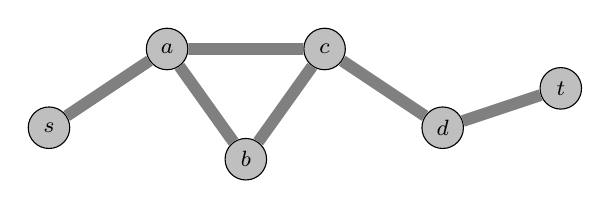
\begin{tikzpicture}
            \tikzstyle{every node}=[circle, fill=lightgray, draw=black, inner sep=2pt, minimum size=1.5em, font=\footnotesize, text=black]
            \tikzstyle{edge}=[gray, line width=1.5mm]
       
            \node (s) at (0.5,1) {$s$};
            \node (a) at (2,2) {$a$};
            \node (b) at (3,0.6) {$b$};
            \node (c) at (4,2) {$c$};
            \node (d) at (5.5,1) {$d$};
            \node (t) at (7,1.5) {$t$};
       
            \draw[edge] (s) -- (a) -- (c) -- (d) -- (t);
            \draw[edge] (a) -- (b) -- (c);
          \end{tikzpicture}
          \caption{The input graph $G$}
          \label{figure:input-graph}
    \end{subfigure}\hfill%
    \begin{subfigure}{.45\textwidth}
        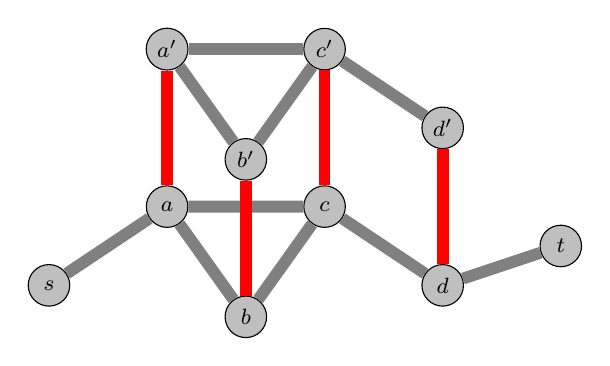
\begin{tikzpicture}
            \tikzstyle{every node}=[circle, fill=lightgray, draw=black, inner sep=2pt, minimum size=1.5em, font=\footnotesize, text=black]
            \tikzstyle{edge}=[gray, line width=1.5mm]
       
            \node (s) at (0.5,1) {$s$};
            \node (a) at (2,2) {$a$};
            \node (b) at (3,0.6) {$b$};
            \node (c) at (4,2) {$c$};
            \node (d) at (5.5,1) {$d$};
            \node (t) at (7,1.5) {$t$};

            \node (a') at (2,4) {$a'$};
            \node (b') at (3,2.6) {$b'$};
            \node (c') at (4,4) {$c'$};
            \node (d') at (5.5,3) {$d'$};
       
            \draw[edge] (s) -- (a) -- (c) -- (d) -- (t);
            \draw[edge] (a) -- (b) -- (c);

            \draw[edge] (a') -- (b') -- (c') -- (d');
            \draw[edge] (a') -- (c');

            \tikzstyle{edge}=[red, line width=1.5mm]
            \draw[edge] (a) -- (a');
            \draw[edge] (b) -- (b');
            \draw[edge] (c) -- (c');
            \draw[edge] (d) -- (d');
        \end{tikzpicture}
        \caption{The mirror graph $H$ of $G$, mirror edges marked in red}
        \label{figure:mirror-graph}
    \end{subfigure}
 \end{figure}

For example, if our input $G$ for \textsc{Shortest Odd Path} is Figure ~\ref{figure:input-graph}, then $H$ and $F$ could look like Figure ~\ref{figure:mirror-graph}. One of the two possible alternating paths is $P' := [(s,a), (a, a'), (a',b'), (b',b)$, $(b,c), (c,c'), (c',d'), (d',d), (d,t)]$. When we filter out mirror edges and replace edges from the mirror side with their real counterparts, we end up with $P := [(s,a),(a,b),(b,c),(c,d),(d,t)]$, which is one of the two possible odd paths of $G$. 
\todo{dette kan kanskje formuleres bedre?}

To see why the reduction works, simply observe that for each step we take in the graph, we have to go to the other side of the mirror. If we take another step, we get back to the same side again. It is only when we reach the target vertex $t$ that we do not have to go to the other side. Therefore, to reach a neighbour of $t$, we must have used an even number of mirror edges and an even number of non-mirror edges, and when we take the last step to reach $t$ we have used an odd number of edges and thus found an odd path. If this alternating $s$-$t$-path in $H$ is the shortest such path, then the corresponding path in $G$ must also be the shortest odd $s$-$t$-path in $G$. The reduction works also in the weighted case, as long as each edge $(u',v')$ on the mirror side get the same weight as their real counterpart, and all the mirror edges get the same (usually 0) weight. The interested reader may see \cite{source:derigs_shortest_odd_path} for more details on this reduction.

Ball and Derigs \cite{source:shortest_alternating_path} have shown how to efficiently solve \textsc{Shortest Alternating Path}. In their algorithms, subgraphs are shrunk into psuedonodes whenever possible, to make the graph smaller. The drawback is that certain psuedonodes must later be expanded again, which is the most complicated and expensive part of their algorithms. In our case, however, we have a special case of \textsc{Shortest Alternating Path}. The set $F$ is, with the exception of $s$ and $t$, a perfect matching of $H$, and we will therefore never have to expand psuedonodes after shrinking them. The curious reader may visit \cite{source:shortest_alternating_path} for more on these algorithms and why our almost-perfect matching is a simpler case.

\subsection{The idea for our \textsc{Shortest Alternating Path} algorithm}
We will explain the general idea of our algorithm by following an example, and solve for the graph in figure \ref{figure:input-graph}. First we construct the mirror graph like explained in \ref{subsection:reduction}, to produce the graph in figure \ref{figure:mirror-graph}. Then we initialize an empty priority queue of vertices and edges to be scanned. For each vertex $u \in V(H)$, we denote
\begin{itemize}
    \item $d^+_u :=$ the length of the shortest alternating $s$-$u$-path ending on a mirror edge
    \item $d^-_u :=$ the length of the shortest alternating $s$-$u$-path ending on a non-mirror edge
    \item $pred_u :=$ the last edge used to find $u$'s most recent value for $d^-_u$
\end{itemize}

Initally these are either $\infty$ or undefined, except for the source vertex $s$, where we can set $d^+_s := 0$. Then, for each edge $(s,u) \in N(s)$, we can set $d^-_u := weight((s,u))$, $pred_u := (s,u)$, and add $u$ to our priority queue with priority $2 \cdot weight((s,u))$.

We visualize it in the diagram below.

\begin{minipage}{.75\linewidth}
    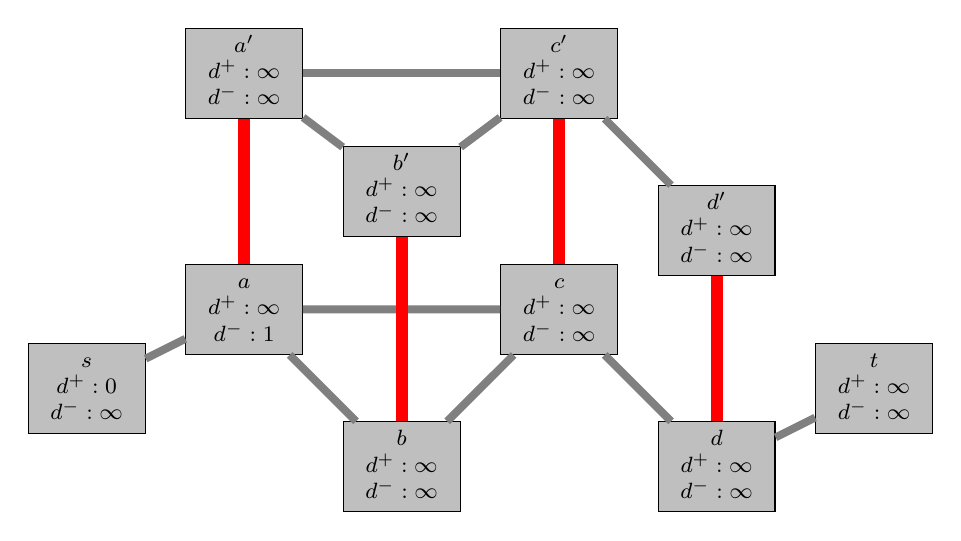
\begin{tikzpicture}{text centered}
        \tikzstyle{every node}=[rectangle, fill=lightgray, draw=black, inner sep=2pt, minimum size=1.5em, font=\footnotesize, text=black]
        \tikzstyle{edge}=[gray, line width=1mm]
   
        \node (s) at (0,1)    {\begin{tabular}{c} $s$  \\ $d^+:0$       \\ $d^-:\infty$ \end{tabular}};
        \node (a) at (2,2)    {\begin{tabular}{c} $a$  \\ $d^+:\infty$  \\ $d^-:1$      \end{tabular}};
        \node (b) at (4,0)    {\begin{tabular}{c} $b$  \\ $d^+:\infty$  \\ $d^-:\infty$ \end{tabular}};
        \node (c) at (6,2)    {\begin{tabular}{c} $c$  \\ $d^+:\infty$  \\ $d^-:\infty$ \end{tabular}};
        \node (d) at (8,0)    {\begin{tabular}{c} $d$  \\ $d^+:\infty$  \\ $d^-:\infty$ \end{tabular}};
        \node (t) at (10,1)   {\begin{tabular}{c} $t$  \\ $d^+:\infty$  \\ $d^-:\infty$ \end{tabular}};

        \node (a') at (2,5)   {\begin{tabular}{c} $a'$ \\ $d^+:\infty$  \\ $d^-:\infty$ \end{tabular}};
        \node (b') at (4,3.5) {\begin{tabular}{c} $b'$ \\ $d^+:\infty$  \\ $d^-:\infty$ \end{tabular}};
        \node (c') at (6,5)   {\begin{tabular}{c} $c'$ \\ $d^+:\infty$  \\ $d^-:\infty$ \end{tabular}};
        \node (d') at (8,3)   {\begin{tabular}{c} $d'$ \\ $d^+:\infty$  \\ $d^-:\infty$ \end{tabular}};
   
        \draw[edge] (s) -- (a) -- (c) -- (d) -- (t);
        \draw[edge] (a) -- (b) -- (c);

        \draw[edge] (a') -- (b') -- (c') -- (d');
        \draw[edge] (a') -- (c');

        \tikzstyle{edge}=[red, line width=1.5mm]
        \draw[edge] (a) -- (a');
        \draw[edge] (b) -- (b');
        \draw[edge] (c) -- (c');
        \draw[edge] (d) -- (d');
    \end{tikzpicture}
\end{minipage}\hfill%
\begin{minipage}{.22\linewidth}
    Queue:
    \begin{itemize}
        \item $\text{Vertex}(2, a)$
    \end{itemize}
\end{minipage}

\includesvg[width=12cm]{figures/example_story/example-story1.svg}

The first and only vertex in the queue is $A$. We pop it, set $d^+_{A'} := d^-_A$, and 'scan' $A'$. By that, we mean to look at each neighbour $e \in N(A')$, and see if our new value $d^+_{A'} + weight(e)$ is better than the previous value $d^-_{to(edge)}$. That is the case for both $B'$ and $C'$, so we update their values and add them to the queue. Their priorities in the queue is equal to twice their $d^-$ values, which is $2 \cdot 2 = 4$ for both of them.

\includesvg[width=12cm]{figures/example_story/example-story2.svg}

The next vertex in the queue is $B'$, so we set $d^+_B := d^-_{B'}$ and scan $B'$:

\includesvg[width=12cm]{figures/example_story/example-story3.svg}

Now $C'$ is the next in the queue, we set $d^+_C := d^-{C'}$ and scan $C'$. This is where the interesting part happens: now we have set both $d^+$ and $d^-$ for $B$ and $C$, and that means that we have found an odd cycle in the graph. The edge between them, $(B,C)$, is called the \emph{blossom edge}, and is marked in green. We add $(B,C)$ to the queue, with the priority $d^+_C + d^+_B + weight((B,C))$.

\includesvg[width=12cm]{figures/example_story/example-story4.svg}

Next up is to scan this blossom edge, and compute its corresponding odd cycle by backtracking from $C$ and $B$ until they meet at $A'$. To visualize the cycle, we like to 'stretch out' the graph a little, and draw it like below. Note that some of the edges are omitted for clarity. Now we can see that the cycle consists of [$A',C',C,B,B',A'$]. We call the set $\mathbb{B} := \{C',C,B,B'\}$ a \emph{blossom}, and $A'$ the \emph{base} of the blossom, inspired by the famous Blossom algorithm by \cite{source:blossom}.

\includesvg[width=12cm]{figures/example_story/example-story5.svg}

The first reason why we care about this blossom is because now we can immedeately set the final, optimal $d^-$ and $d^+$ for all the vertices in the blossom. That is because we now have two alternating paths to each vertex, one goes around the cycle while the other takes the shortcut. One of these ends up on a mirror edge, and the other on a normal edge, and both are optimal. For example, to go from $S$ to $C'$, we can either go through [$S,A,A',C'$] with a cost of $d^-_C$, or go along [$S,A,A',B',B,C,C'$] with a cost of $d^+_C$.

More specifically, for each $u \in \mathbb{B}$: \begin{itemize}
    \item If $d^+_u = \infty$, we set $d^+_u = d^-_{mirror(u)}$.
    \item If we can improve $d^-_u$ by coming from its neighbour in the blossom, we do so.
\end{itemize}
After all these values have been set, we immedeately scan all the vertices in $\mathbb{B}$ that just received values for $d^+$. In this example we scan $C'$ and $B'$, and discover $D'$. Unfortunately, since this is a very small blossom we don't have any vertices that receive new values for $d^-$.

\includesvg[width=12cm]{figures/example_story/example-story6.svg}

\todo{føler dette kan skrives bedre}
The second reason we compute the blossom is that we no longer care much about the individual vertices in $\mathbb{B}$, and can shrink it into just the base $A'$. We will still scan vertices like $C$ from the queue as before, but whenever we are backtracking to compute blossoms we can skip the verties in $\mathbb{B}$ entirely and go straight to the base $A'$ instead. In this example, in a few iterations the algorithm will find either $(D',A')$ or $(D,A')$ as a blossom edge, with just $\{D,D'\}$ as its blossom and $A'$ as the base here as well. If we didn't contract the previous blossom, this new blossom would instead consist of $\{C',C,B,B',D,D'\}$, but we are already completely done with most of those vertices and computing all of it again would be a waste. Therefore we shrink them. 

If the reader is familiar with the more general \textsc{Shortest Alternating Path} algorithm \cite{source:shortest_alternating_path} or the original blossom algorithm \cite{source:blossom}, and worry that such psuedonodes often have to be expanded again, then remember that in our case the set $F$ is an almost-perfect matching and those cases never happen. \todo{trenger vi si dette? Droppe det? Formulere det annerledes?}

\includesvg[width=12cm]{figures/example_story/example-story7.svg}

Let us now skip a few steps, until $T$ eventually reaches the front of the queue. At that point we have that $d^-_T = 5$, and that is also the cost of the shortest odd path in our original input graph. To compute the exact path we can backtrack from $T$ to $S$ and then translate that path as described in step \ref{point:translate_alternating_path} of our reduction in \ref{subsection:reduction}. We end up with the path [$(S,A),(A,B),(B,C),(C,D),(D,T)$], which is the shortest odd $S$-$T$-path in the graph.
